% Options for packages loaded elsewhere
\PassOptionsToPackage{unicode}{hyperref}
\PassOptionsToPackage{hyphens}{url}
\documentclass[
]{article}
\usepackage{xcolor}
\usepackage{amsmath,amssymb}
\setcounter{secnumdepth}{5}
\usepackage{iftex}
\ifPDFTeX
  \usepackage[T1]{fontenc}
  \usepackage[utf8]{inputenc}
  \usepackage{textcomp} % provide euro and other symbols
\else % if luatex or xetex
  \usepackage{unicode-math} % this also loads fontspec
  \defaultfontfeatures{Scale=MatchLowercase}
  \defaultfontfeatures[\rmfamily]{Ligatures=TeX,Scale=1}
\fi
% \usepackage{lmodern}
\ifPDFTeX\else
  % xetex/luatex font selection
\fi
% Use upquote if available, for straight quotes in verbatim environments
\IfFileExists{upquote.sty}{\usepackage{upquote}}{}
\IfFileExists{microtype.sty}{% use microtype if available
  \usepackage[]{microtype}
  \UseMicrotypeSet[protrusion]{basicmath} % disable protrusion for tt fonts
}{}
\makeatletter
\@ifundefined{KOMAClassName}{% if non-KOMA class
  \IfFileExists{parskip.sty}{%
    \usepackage{parskip}
  }{% else
    \setlength{\parindent}{0pt}
    \setlength{\parskip}{6pt plus 2pt minus 1pt}}
}{% if KOMA class
  \KOMAoptions{parskip=half}}
\makeatother
\usepackage{color}
\usepackage{fancyvrb}
\newcommand{\VerbBar}{|}
\newcommand{\VERB}{\Verb[commandchars=\\\{\}]}
\DefineVerbatimEnvironment{Highlighting}{Verbatim}{commandchars=\\\{\}}
% Add ',fontsize=\small' for more characters per line
\newenvironment{Shaded}{}{}
\newcommand{\AlertTok}[1]{\textcolor[rgb]{1.00,0.00,0.00}{\textbf{#1}}}
\newcommand{\AnnotationTok}[1]{\textcolor[rgb]{0.38,0.63,0.69}{\textbf{\textit{#1}}}}
\newcommand{\AttributeTok}[1]{\textcolor[rgb]{0.49,0.56,0.16}{#1}}
\newcommand{\BaseNTok}[1]{\textcolor[rgb]{0.25,0.63,0.44}{#1}}
\newcommand{\BuiltInTok}[1]{\textcolor[rgb]{0.00,0.50,0.00}{#1}}
\newcommand{\CharTok}[1]{\textcolor[rgb]{0.25,0.44,0.63}{#1}}
\newcommand{\CommentTok}[1]{\textcolor[rgb]{0.38,0.63,0.69}{\textit{#1}}}
\newcommand{\CommentVarTok}[1]{\textcolor[rgb]{0.38,0.63,0.69}{\textbf{\textit{#1}}}}
\newcommand{\ConstantTok}[1]{\textcolor[rgb]{0.53,0.00,0.00}{#1}}
\newcommand{\ControlFlowTok}[1]{\textcolor[rgb]{0.00,0.44,0.13}{\textbf{#1}}}
\newcommand{\DataTypeTok}[1]{\textcolor[rgb]{0.56,0.13,0.00}{#1}}
\newcommand{\DecValTok}[1]{\textcolor[rgb]{0.25,0.63,0.44}{#1}}
\newcommand{\DocumentationTok}[1]{\textcolor[rgb]{0.73,0.13,0.13}{\textit{#1}}}
\newcommand{\ErrorTok}[1]{\textcolor[rgb]{1.00,0.00,0.00}{\textbf{#1}}}
\newcommand{\ExtensionTok}[1]{#1}
\newcommand{\FloatTok}[1]{\textcolor[rgb]{0.25,0.63,0.44}{#1}}
\newcommand{\FunctionTok}[1]{\textcolor[rgb]{0.02,0.16,0.49}{#1}}
\newcommand{\ImportTok}[1]{\textcolor[rgb]{0.00,0.50,0.00}{\textbf{#1}}}
\newcommand{\InformationTok}[1]{\textcolor[rgb]{0.38,0.63,0.69}{\textbf{\textit{#1}}}}
\newcommand{\KeywordTok}[1]{\textcolor[rgb]{0.00,0.44,0.13}{\textbf{#1}}}
\newcommand{\NormalTok}[1]{#1}
\newcommand{\OperatorTok}[1]{\textcolor[rgb]{0.40,0.40,0.40}{#1}}
\newcommand{\OtherTok}[1]{\textcolor[rgb]{0.00,0.44,0.13}{#1}}
\newcommand{\PreprocessorTok}[1]{\textcolor[rgb]{0.74,0.48,0.00}{#1}}
\newcommand{\RegionMarkerTok}[1]{#1}
\newcommand{\SpecialCharTok}[1]{\textcolor[rgb]{0.25,0.44,0.63}{#1}}
\newcommand{\SpecialStringTok}[1]{\textcolor[rgb]{0.73,0.40,0.53}{#1}}
\newcommand{\StringTok}[1]{\textcolor[rgb]{0.25,0.44,0.63}{#1}}
\newcommand{\VariableTok}[1]{\textcolor[rgb]{0.10,0.09,0.49}{#1}}
\newcommand{\VerbatimStringTok}[1]{\textcolor[rgb]{0.25,0.44,0.63}{#1}}
\newcommand{\WarningTok}[1]{\textcolor[rgb]{0.38,0.63,0.69}{\textbf{\textit{#1}}}}
\usepackage{longtable,booktabs,array}
\newcounter{none} % for unnumbered tables
\usepackage{calc} % for calculating minipage widths
% Correct order of tables after \paragraph or \subparagraph
\usepackage{etoolbox}
\makeatletter
\patchcmd\longtable{\par}{\if@noskipsec\mbox{}\fi\par}{}{}
\makeatother
% Allow footnotes in longtable head/foot
\IfFileExists{footnotehyper.sty}{\usepackage{footnotehyper}}{\usepackage{footnote}}
\makesavenoteenv{longtable}
\usepackage{graphicx}
\makeatletter
\newsavebox\pandoc@box
\newcommand*\pandocbounded[1]{% scales image to fit in text height/width
  \sbox\pandoc@box{#1}%
  \Gscale@div\@tempa{\textheight}{\dimexpr\ht\pandoc@box+\dp\pandoc@box\relax}%
  \Gscale@div\@tempb{\linewidth}{\wd\pandoc@box}%
  \ifdim\@tempb\p@<\@tempa\p@\let\@tempa\@tempb\fi% select the smaller of both
  \ifdim\@tempa\p@<\p@\scalebox{\@tempa}{\usebox\pandoc@box}%
  \else\usebox{\pandoc@box}%
  \fi%
}
% Set default figure placement to htbp
\def\fps@figure{htbp}
\makeatother
\setlength{\emergencystretch}{3em} % prevent overfull lines
\providecommand{\tightlist}{%
  \setlength{\itemsep}{0pt}\setlength{\parskip}{0pt}}
\usepackage[]{natbib}
\bibliographystyle{plainnat}
\makeatletter
\@ifpackageloaded{subcaption}{}{\usepackage{subcaption}}
\@ifpackageloaded{caption}{}{\usepackage{caption}}
\captionsetup[subfigure]{margin=0.5em}
\AtBeginDocument{%
\renewcommand*\figurename{Figure}
\renewcommand*\tablename{Table}
}
\AtBeginDocument{%
\renewcommand*\listfigurename{List of Figures}
\renewcommand*\listtablename{List of Tables}
}
\newcounter{pandoccrossref@subfigures@footnote@counter}
\newenvironment{pandoccrossrefsubfigures}{%
\setcounter{pandoccrossref@subfigures@footnote@counter}{0}
\begin{figure}\centering%
\gdef\global@pandoccrossref@subfigures@footnotes{}%
\DeclareRobustCommand{\footnote}[1]{\footnotemark%
\stepcounter{pandoccrossref@subfigures@footnote@counter}%
\ifx\global@pandoccrossref@subfigures@footnotes\empty%
\gdef\global@pandoccrossref@subfigures@footnotes{{##1}}%
\else%
\g@addto@macro\global@pandoccrossref@subfigures@footnotes{, {##1}}%
\fi}}%
{\end{figure}%
\addtocounter{footnote}{-\value{pandoccrossref@subfigures@footnote@counter}}
\@for\f:=\global@pandoccrossref@subfigures@footnotes\do{\stepcounter{footnote}\footnotetext{\f}}%
\gdef\global@pandoccrossref@subfigures@footnotes{}}
\@ifpackageloaded{float}{}{\usepackage{float}}
\floatstyle{ruled}
\@ifundefined{c@chapter}{\newfloat{codelisting}{h}{lop}}{\newfloat{codelisting}{h}{lop}[chapter]}
\floatname{codelisting}{Listing}
\newcommand*\listoflistings{\listof{codelisting}{List of Listings}}
\makeatother
\usepackage{bookmark}
\IfFileExists{xurl.sty}{\usepackage{xurl}}{} % add URL line breaks if available
\urlstyle{same}
% fallback for those not using the hyperref driver hyperxmp:
\makeatletter
\@ifundefined{xmpquote}{\newcommand{\xmpquote}[1]{#1}}{}
\makeatother
\hypersetup{
  colorlinks=true,linkcolor=red,urlcolor=red,citecolor=red,anchorcolor=red,filecolor=red,
  pdfcreator={LaTeX via pandoc}}

\author{}
\date{}

\IfFileExists{seqsplit.sty}{\usepackage{seqsplit}}{\newcommand{\seqsplit}[1]{#1}}
\protected\def\breakseq#1{\seqsplit{#1}}
\protected\def\breaktt#1{\begingroup\ttfamily\seqsplit{#1}\endgroup}
\title{Active Inference -- A Synthetic Overview}
\author{Daniel Ari Friedman\\\footnotesize{Active Inference Institute}\\\footnotesize{\texttt{daniel@activeinference.institute}}\\\footnotesize{\href{https://orcid.org/0000-0001-6232-9096}{ORCID: 0000-0001-6232-9096}} \\and Alexandra Mikhailova\\\footnotesize{Active Inference Institute}\\\footnotesize{\texttt{alexandra@activeinference.institute}}}
\date{2026-06-28}

% Core mathematics
\usepackage{amsmath}
\usepackage{amssymb}
\usepackage{amsfonts}
\usepackage{amsthm}

% Document layout
\usepackage{geometry}
\geometry{margin=0.25in}
\usepackage{float}
\usepackage{graphicx}

% Tables
\usepackage{booktabs}
\usepackage{longtable}
\usepackage{array}

% Algorithm typesetting (for pseudocode in §2 Methodology)
\usepackage[ruled,vlined,linesnumbered]{algorithm2e}

% Code listings
\usepackage{listings}

% Typography and formatting
\usepackage{microtype}
\usepackage{xcolor}
\usepackage[binary-units]{siunitx}

% Cross-references and citations
\usepackage{hyperref}
\hypersetup{
    colorlinks=true,
    allcolors=red
}
\usepackage[capitalise,noabbrev]{cleveref}
\usepackage{natbib}

% ── Unicode-capable mono font for code listings ──────────────────────
% JuliaMono (TeX Live 2026) covers the full math/Greek glyph set used in
% scientific code blocks; the default lmmono lacks \alpha/\mu/\partial/\nabla.
%
% The hardcoded TeX Live 2026 path below is portable to most macOS / Linux
% TeX Live installs that placed JuliaMono under the default texmf-dist path.
% If your TeX Live version differs (e.g., 2025, 2027) or your distribution
% installs fonts elsewhere, comment out the explicit Path = line — fontspec
% will then search the system font path. If JuliaMono is not installed at
% all, comment out the whole block; xelatex falls back to lmmono with
% reduced Unicode coverage but the document still compiles.
\usepackage{fontspec}
\setmonofont{JuliaMono-Regular}[
  Path           = /usr/local/texlive/2026/texmf-dist/fonts/truetype/public/juliamono/,
  Extension      = .ttf,
  UprightFont    = *,
  BoldFont       = JuliaMono-Bold,
  ItalicFont     = JuliaMono-RegularItalic,
  BoldItalicFont = JuliaMono-BoldItalic,
  Scale          = MatchLowercase,
]

% Math font for unicode-math: Latin Modern Math (TeX Live) has full BMP
% coverage including U+2223 (\mid), U+226A/226B (\ll/\gg), and the Greek/
% blackboard letters used in equations. Without an explicit \setmathfont,
% unicode-math falls back to lmroman text font which lacks several glyphs
% and emits "Missing character" warnings on every \mid in math mode.
\setmathfont{latinmodern-math.otf}

\begin{document}

\begin{titlepage}
\centering
\vspace*{2cm}
{\LARGE\bfseries Active Inference -- A Synthetic Overview\par}
\vspace{0.75em}
{\large An applicable introduction across equilibrium and far-from-equilibrium systems\par}
\vfill
\makeatletter
{\@author\par}
\vspace{1em}
{\@date\par}
\makeatother
\vfill
\end{titlepage}
\thispagestyle{empty}
\tableofcontents
\newpage


\section{Abstract}\label{sec:abstract}

Active Inference casts perception and action as free-energy
minimization. This overview shows how Bayesian mechanics carries the
Free Energy Principle from equilibrium to far-from-equilibrium life.

\newpage

\section{Extended Abstract}\label{sec:extended}

A thing that persists must, in effect, hold a model of the world that
keeps it intact. \textbf{Active Inference} turns that observation into
mechanics: a system maintains itself by minimizing \emph{variational
free energy}, a single quantity that scores how badly its internal
expectations fit incoming sensations
\citep{friston2010fep, parr2022active}. Perception lowers free energy by
updating beliefs; action lowers it by changing the world so the beliefs
come true. One currency, two directions --- inference and control ---
which is why the same template reappears from single cells to brains to
institutions.

The bound is what makes this \emph{applicable} rather than metaphorical.
Variational free energy is an upper bound on \textbf{surprise}, the
negative log evidence \(-\ln p(s)\) a system assigns to its own sensory
states. Because the bound is computable from a system's own beliefs,
minimizing it \emph{is} approximate Bayesian inference carried out by
the physical dynamics of the thing itself. The accounting is organized
by a \textbf{Markov blanket}: a statistical boundary splitting
\emph{external} states \(\eta\) from \emph{internal} states \(\mu\),
coupled only through \emph{sensory} and \emph{active} blanket states.
Internal states come to parameterize beliefs about the external world
they can never touch directly --- the core claim of \textbf{Bayesian
mechanics}, a physics written in terms of, and by, those beliefs
\citep{dacosta2021bayesian, ramstead2023bayesian}.

fig.~\ref{fig:overview} shows the move that this overview is built
around, without a single equation of derivation. Both panels live on
\emph{the same} free-energy landscape --- a Gaussian bowl whose floor is
the system's expected state. At \textbf{equilibrium} (panel a) the flow
is pure descent, \(f=-\nabla F\): every trajectory falls straight to the
mode and stops. Detailed balance holds, there is no net current, and ---
taken literally --- nothing further happens. A rock is at equilibrium;
so, eventually, is a system that has stopped doing anything. Living
systems occupy panel (b). There the flow gains a \emph{solenoidal} term,
\(f=(Q-\Gamma)\nabla F\), that runs along the contours of \(F\) rather
than down them. Free energy is still minimized --- the system still
tracks its niche --- yet probability mass \textbf{circulates}
indefinitely in a \textbf{non-equilibrium steady state}. That persistent
current is the signature of things that stay far from equilibrium:
heartbeats, foraging, perception that never settles. The gradient part
is the Free Energy Principle's ``climbing down surprise''; the
solenoidal part is what keeps the system alive while doing so
\citep{friston2023bayesian}.

Read the two panels together and the headline of Active Inference is
visible at a glance: the \emph{same} imperative --- minimize free energy
--- produces inert relaxation in one regime and open-ended,
self-sustaining behavior in the other. The rest of this overview unpacks
that picture in the spirit of \emph{show, not tell}: each subsequent
section adds one runnable, minimal demonstration rather than another
layer of formalism.

\begin{figure}
\centering
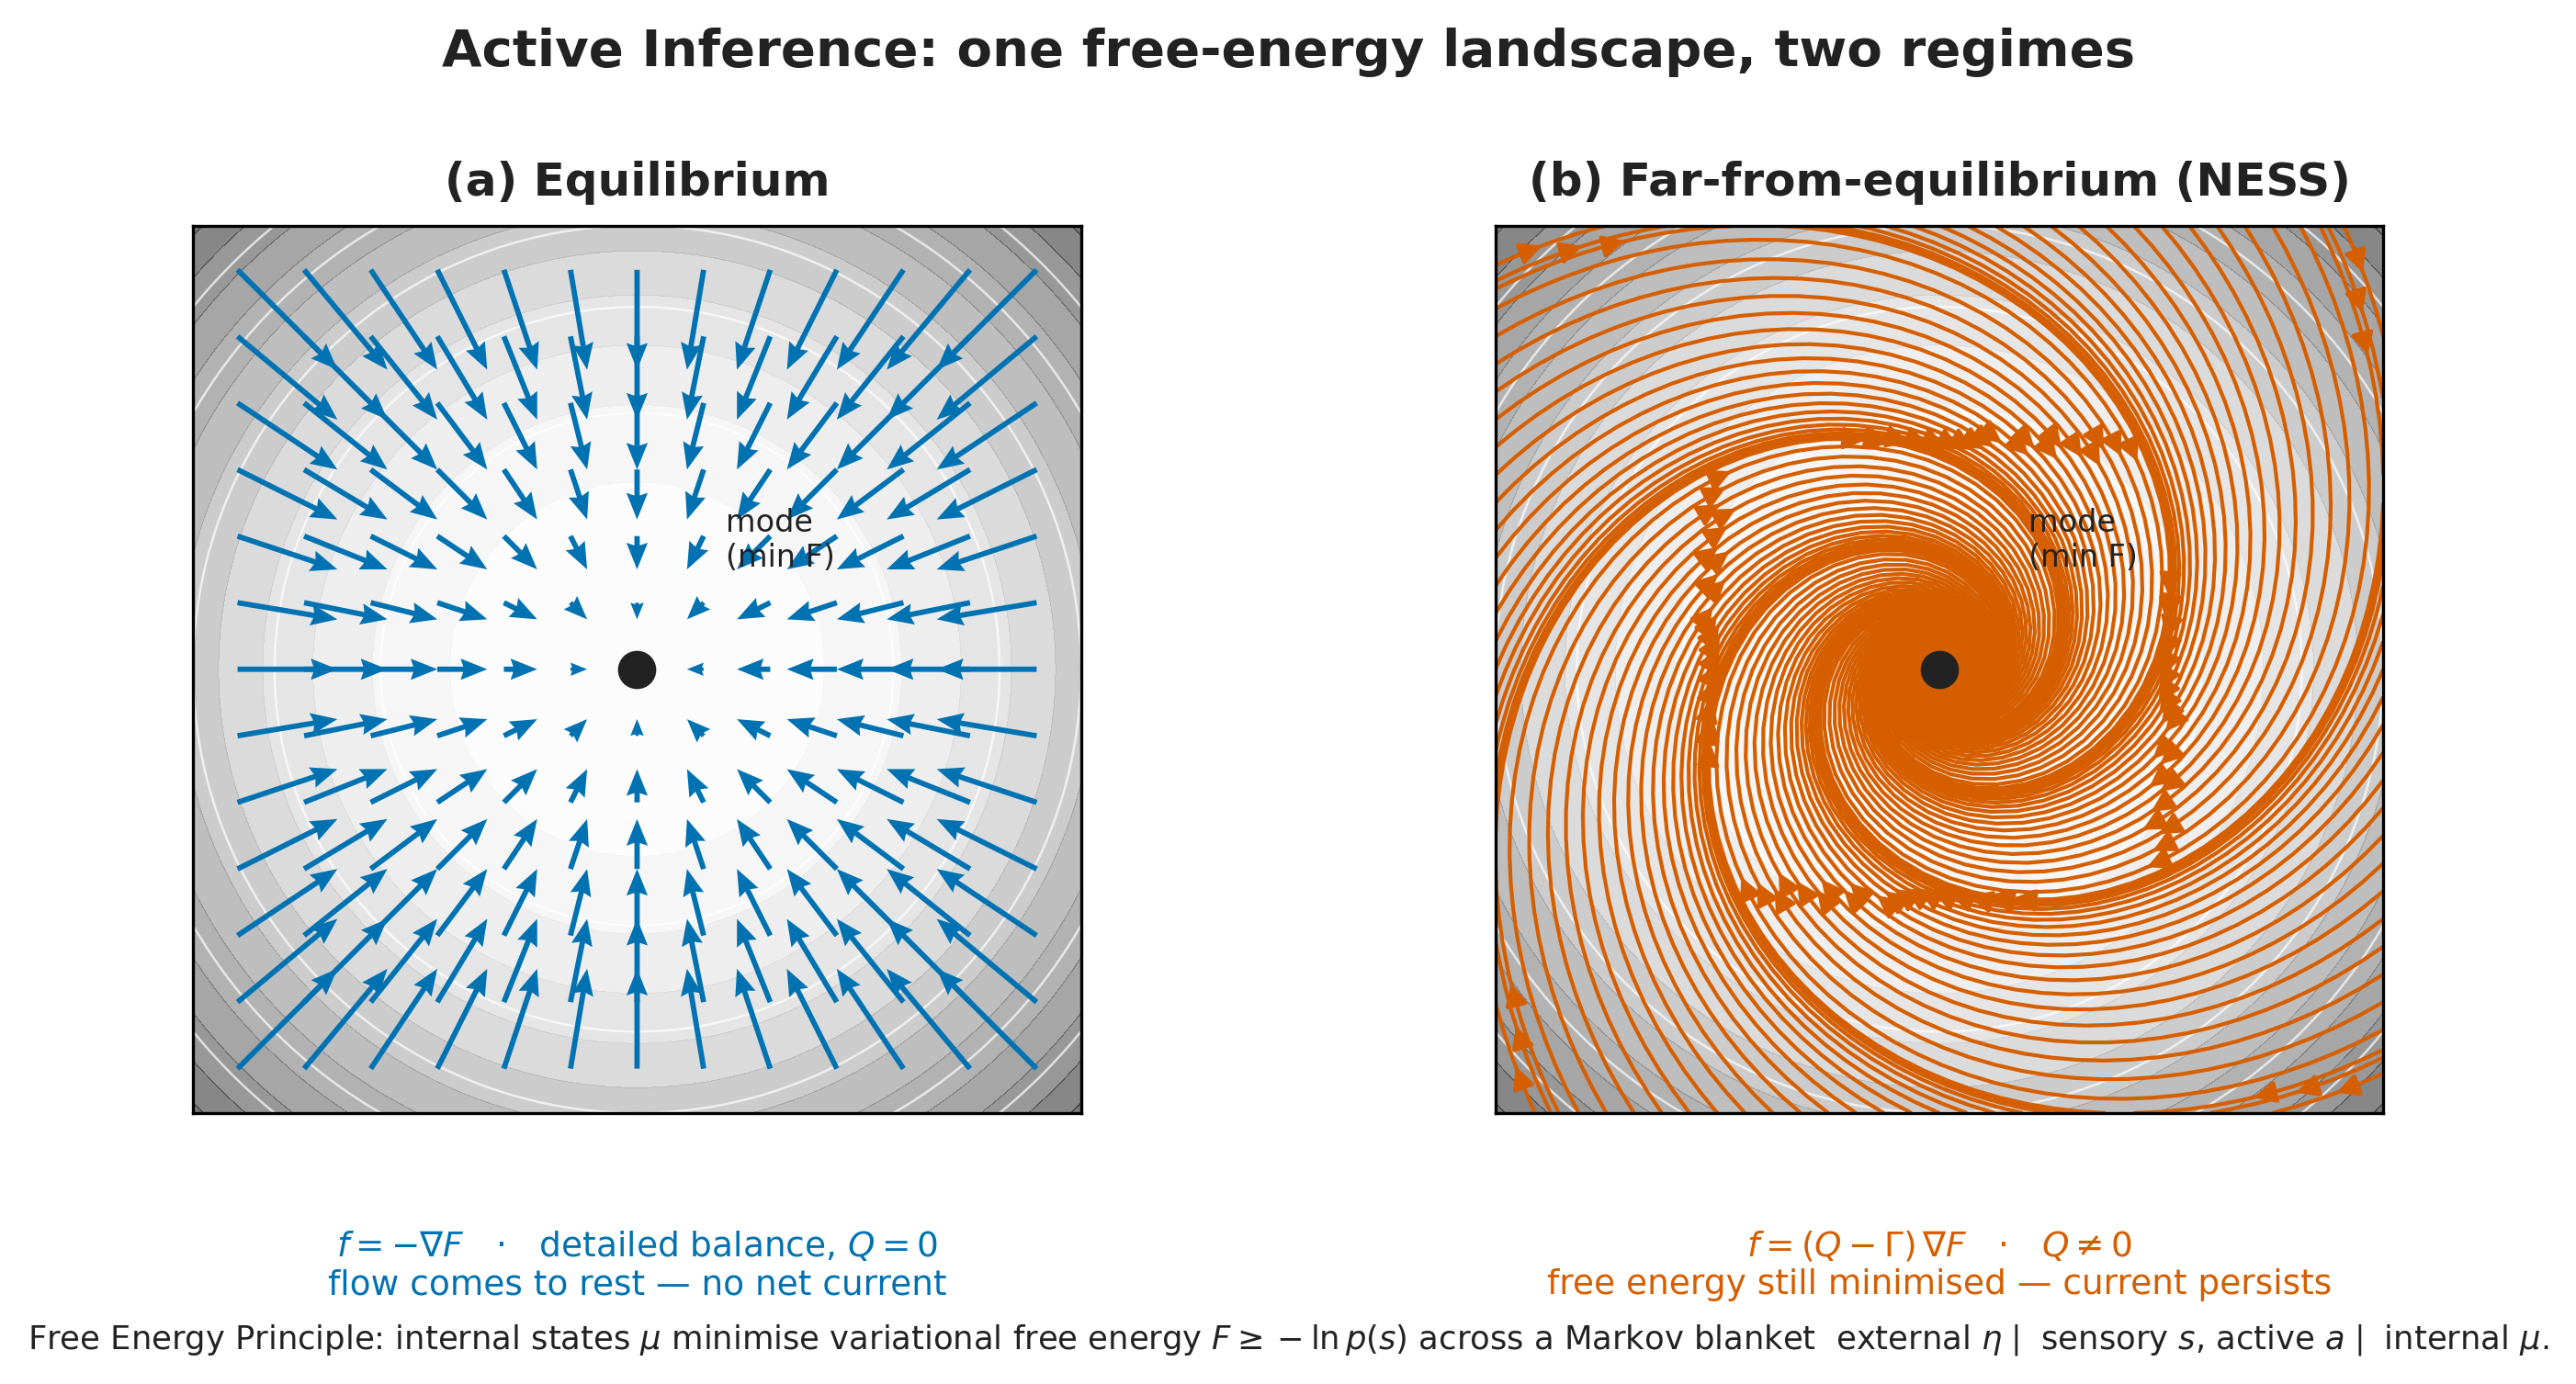
\includegraphics[width=0.94\linewidth,height=0.50\textheight,keepaspectratio,alt={One landscape, two regimes. Both panels place the system on the same Gaussian free-energy bowl (grey contours; the black dot marks the mode, where free energy is least). (a) Equilibrium: the flow is pure gradient descent on free energy, f=-\textbackslash nabla F (blue arrows). Detailed balance holds, so trajectories fall to the mode and come to rest with no net probability current. (b) Far-from-equilibrium (NESS): an antisymmetric solenoidal operator Q adds a conservative current, f=(Q-\textbackslash Gamma)\textbackslash nabla F (orange streamlines), that flows along the level sets of F. Free energy is still minimized, but probability mass circulates without end --- the hallmark of living, self-organizing systems. The Free Energy Principle is the descent term; Bayesian mechanics adds the circulation. Internal states \textbackslash mu infer external states \textbackslash eta across a Markov blanket (sensory s, active a). Figure rendered deterministically by scripts/generate\_overview\_figure.py over the tested flow in src/free\_energy\_flow.py.}]{../figures/active_inference_overview.png}
\caption{\textbf{One landscape, two regimes.} Both panels place the
system on the same Gaussian free-energy bowl (grey contours; the black
dot marks the mode, where free energy is least). \textbf{(a)
Equilibrium:} the flow is pure gradient descent on free energy,
\(f=-\nabla F\) (blue arrows). Detailed balance holds, so trajectories
fall to the mode and come to rest with no net probability current.
\textbf{(b) Far-from-equilibrium (NESS):} an antisymmetric
\emph{solenoidal} operator \(Q\) adds a conservative current,
\(f=(Q-\Gamma)\nabla F\) (orange streamlines), that flows along the
level sets of \(F\). Free energy is still minimized, but probability
mass circulates without end --- the hallmark of living, self-organizing
systems. The Free Energy Principle is the descent term; Bayesian
mechanics adds the circulation. Internal states \(\mu\) infer external
states \(\eta\) across a Markov blanket (sensory \(s\), active \(a\)).
Figure rendered deterministically by
\protect\breaktt{scripts/generate\_overview\_figure.py} over the tested
flow in \protect\breaktt{src/free\_energy\_flow.py}.}\label{fig:overview}
\end{figure}

\newpage

\section{References}\label{sec:references}

Bibliography lives in
\href{references.bib}{\breaktt{manuscript/references.bib}} and is read by
Pandoc during PDF render. The build pipeline invokes Pandoc with
\texttt{-\/-natbib}, so every \texttt{{[}@key{]}} citation in the
manuscript is rewritten to the appropriate
\texttt{\textbackslash{}cite\{\}}/\texttt{\textbackslash{}citep\{\}}/\texttt{\textbackslash{}citet\{\}}
LaTeX command and resolved against the bib file.

To validate that \texttt{references.bib} is syntactically clean and
contains the required fields per entry type:

\begin{Shaded}
\begin{Highlighting}[]
\ExtensionTok{uv}\NormalTok{ run python }\AttributeTok{{-}m}\NormalTok{ infrastructure.reference.citation.cli validate }\DataTypeTok{\textbackslash{}}
\NormalTok{    projects/working/ActiveInferenceSynthetic/manuscript/references.bib }\AttributeTok{{-}{-}strict}
\end{Highlighting}
\end{Shaded}




\clearpage

\bibliography{references}
\end{document}
